\clearpage %%% für Druck

\subsubsection{Unified Process und Rational Unified Process}
\label{sec:Kap-2.2.2.1}

\vspace{\baselineskip} %%% für Druck

\sttpLeserfuehrung{Bilder/Kapitel-2/Leserfuehrung/vorgehensmodelle_iterativ_inkrementell_illustration.pdf}{Bilder/Kapitel-2/Leserfuehrung/vorgehensmodelle_rational_unified_process.pdf}

Ein  Kritikpunkt am Wasserfallmodell (und anderen Modellen der 1980er Jahre) war die starke Fokussierung auf rein softwaretechnische Aspekte und der damit niedrige Stellenwert der fachlichen Belange des Anwendungsbereichs des zu erstellenden Softwareprodukts. Das betraf den Einbezug zukünftiger Nutzer des Softwareprodukts ebenso wie den Umgang mit sich ändernden oder neuen Anforderungen aus der Domäne. Der Ende der 1990er Jahre im Zusammenhang mit der Unified Modelling Language (UML) entstandene und speziell auf objektorientierte Softwareentwicklung ausgerichtete Unified Software Development Process (kurz: Unified Process) \cite{jac99} legte den Fokus erstmals auf die Domäne und die Erfassung der dortigen Geschäftsprozesse. Der Unified Process selber ist ein sehr allgemein gehaltenes Vorgehensmodell, das zwar die Struktur des Vorgehens vorgibt, in den Details aber sehr unterschiedlich ausgestaltet werden kann. Von den verschiedenen Ausgestaltungen des Unified Process ist der Rational Unified Process die bekannteste Version.

Der von der Firma Rational Software (seit 2003 zu IBM gehörig) entwickelte Rational Unified Process (RUP) ist eine stark ausdifferenzierte und werkzeuggestützte Version des Unified Process. Er ist nicht nur ein Vorgehensmodell, sondern auch eine eigenständige Software-Suite, die verschiedene Entwicklungswerkzeuge anbietet, die auf Grundlage des Vorgehensmodells den Entwicklungsprozess eines konkreten Softwareentwicklungsprojekts unterstützen. 

\minisec{Struktur des Softwareentwicklungsprozesses}

Abbildung~\ref{fig:struktur_des_RUP} zeigt die Struktur des RUP. Der RUP unterscheidet die vier in der Abbildung in den Spalten dargestellten Phasen Konzeption (engl. inception), Ausarbeitung (elaboration), Konstruktion (construction) und Übergang in den Betrieb (transition), die nacheinander stattfinden. Jede Phase ist wiederum in Teilphasen (explizit \textit{Iterationen} \marginline{Iterationen}
genannt) aufgeteilt. Die Anzahl der Iterationen pro Phase ist nicht vorgegeben, sondern abhängig vom konkreten Softwareentwicklungsprojekt; die in der Abbildung dargestellte Anzahl der Iterationen daher nur beispielhaft. Im Gegensatz zu den Phasen eines Wasserfallmodells handelt es sich bei den RUP-Phasen nicht um die Prozesse des Softwareengineering, sondern um eine Aufteilung der Entwicklung in vier große Abschnitte, die jeweils mit Meilensteinen abgeschlossen werden und Auskunft über den Stand der Produktenwicklung geben. Die Prozesse des Softwareengineering bildet der RUP in sogenannten Disziplinen (engl. disciplines; in der Abbildung in den Zeilen dargestellt) ab. Hier werden die Prozesse Geschäftsprozessmodellierung (Business Modeling), Anforderungsermittlung (Requirements), Analyse und Entwurf (Analysis and Design), Implementierung (Implementation), Test (Test) und Auslieferung/Inbetriebnahme (Deployment) als sogenannte \textit{Kerndisziplinen}  sowie die \textit{unterstützenden Disziplinen} 
\marginline{Kerndisziplinen, unterstützende Disziplinen}
Konfigurations- und Änderungs\-manage\-ment (Configuration and Change Management), Projekt\-manage\-ment (Project Manage\-ment) und Entwicklungsinfrastruktur (Environment) unterschieden.

\vspace{-2mm} %%% für Druck

\begin{figure}[h!]
	\centering
	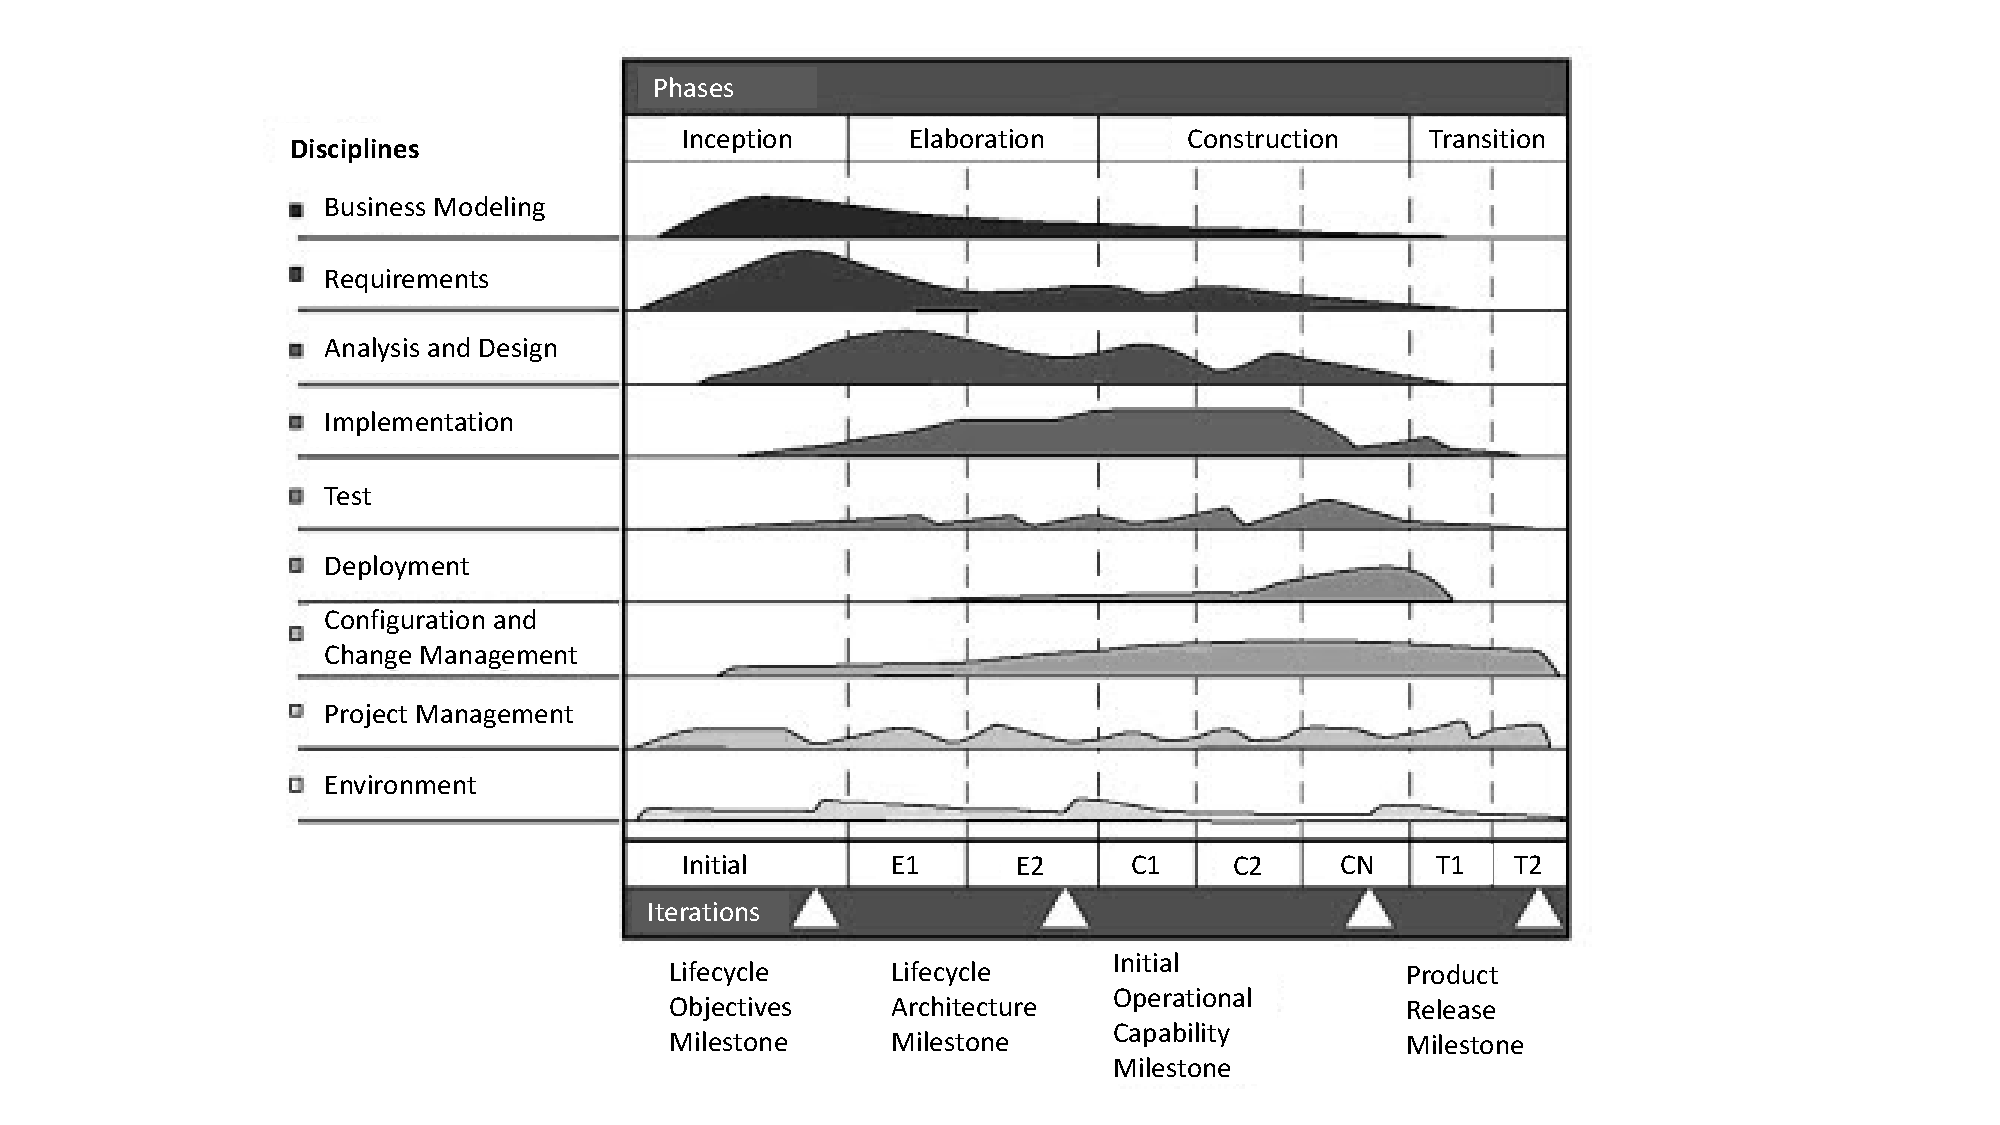
\includegraphics[width=\textwidth]{Bilder/Kapitel-2/StrukturRUP.pdf}
	\caption[Struktur des Rational Unified Process]{Struktur des Rational Unified Process, nach \cite[8]{shu08}}
	\label{fig:struktur_des_RUP}
\end{figure}

\vspace{-2mm} %%% für Druck

Der RUP adressiert mit den drei letztgenannten unterstützenden Disziplinen explizit auch diejenigen Aufgaben, die in einem Softwareentwicklungsprojekt außerhalb der reinen softwaretechnischen Prozesse durchzuführen sind. Innerhalb der Disziplin Projektmanagement nehmen dabei die Durchführung von Machbarkeitsstudien und Wirtschaftlichkeitsprüfungen, aber auch die Verwaltung von Risiko\-management\-plänen einen deutlich höheren Stellenwert ein als bei vielen anderen Vorgehensmodellen. Die Disziplin Entwicklungsinfrastruktur beinhaltet alle Aspekte, die die Bereitstellung von Hardware und Software für das Entwicklungsprojekt betreffen. Die Disziplin Konfigurations- und Änderungsmanagement beinhaltet Aufgaben, die sicherstellen, dass die im Projekt erstellten Dokumente verwaltet und ihre Konsistenz gewährleistet wird. Dazu gehört auch die Pflege einer Versionshistorie. 

In jeder Iteration sollen alle Disziplinen durchlaufen werden, allerdings mit verschiedener Schwerpunktsetzung. Dies verdeutlicht die Abbildung durch die unterschiedlich (und nur idealtypisch) verlaufenden Kurven in den Zeilen der Disziplinen. Je mehr Fläche unterhalb einer Kurve eingezeichnet ist, desto mehr Aufgaben aus dem Bereich der entsprechenden Disziplin werden während der jeweiligen Iteration durchgeführt. So haben zum Beispiel die Disziplinen Geschäftsprozessmodellierung und Anforderungsermittlung ihren Schwerpunkt in der Phase Konzeption, während die Implementierung hauptsächlich zum Ende der Ausarbeitung sowie während der Konstruktionsphase stattfindet. Im Vergleich zu Wasserfallmodellen ist somit nicht jeder Softwareengineering-Prozess fest zugeordnet, sondern wird in jeder Phase (wiederholt) durchlaufen. Insbesondere auch die bei Wasserfallmodellen kritisierte Ver\-ortung von Testaktivitäten löst der RUP dadurch besser. Eine gewisse Ähnlichkeit mit sequentiellen Vorgehensmodellen besteht allerdings doch, da die Schwerpunktsetzung der Kerndisziplinen in den Phasen der aus den sequentiellen Modellen bekannten Reihenfolge Anforderungsermittlung-""Entwurf-""Implementierung-""Testen folgt, auch wenn beim RUP grundsätzlich alle Disziplinen in allen Phasen aktiv sind. Auch Meilensteine am Ende von Phasen sind Charakteristika eines sequen\-tiel\-len Vorgehens, wobei die konkrete Ausgestaltung der Meilensteine im RUP (ausführbarer Architekturprototyp am Ende der zweiten Phase und Beta-Version des Softwareprodukts am Ende der dritten Phase) dann doch eher untypisch sind für sequentielles Vorgehen. 

\vspace{2mm} %%% für Druck

\minisec{Umgang mit Anforderungen}

Im  Vergleich zu vielen anderen Vorgehensmodellen werden im RUP zu Beginn eines Entwicklungsprojekts intensiv die durch das zu entwickelnde Softwareprodukt durchzuführenden oder zu unterstützenden Geschäftsprozesse der Domäne betrachtet. Innerhalb der Disziplin Geschäftsprozessmodellierung werden dafür mithilfe von Anwendungsfall\-mo\-dellen der UML %\sttpkapitelverweis{An\-wen\-dungs\-fall\-mo\-del\-le}{Kap.~\ref{sec:Kap-6.2.1}}
die relevanten Prozesse der Domäne dokumentiert oder auch spezifiziert, falls es sich um zu verändernde oder neu zu schaffende Geschäftsprozesse handelt. Das erfordert eine starke Einbindung der zukünftigen Nutzer des Softwareprodukts, da in der Regel nur diese die vertiefte Kenntnis über die Domäne besitzen. Die erstellten Anwendungsfallmodelle sind eine zentrale Grundlage für die Ermittlung bzw. zum Verständnis der funktionalen Anforderungen 
%\sttpkapitelverweis{funktionale Anforderungen}{Kap.~\ref{sec:Kap-6.1.3.2}}
des zu entwickelnden Softwareprodukts.

Im Rahmen der Disziplin Konfigurations- und Änderungsmanagement werden die Verfahrensweisen für den Umgang mit neuen oder sich ändernden Anforderungen während der Projektlaufzeit festgelegt. Der RUP ist deutlich flexibler bezüglich neuer Anforderungen als sequentielle Modelle, da über das definierte Änderungs\-management auch in späteren Projektphasen grundsätzlich noch Anforderungsänderungen möglich sind. Weitgehende Ergänzungen oder Änderungen der Anforderungen werden aber in der Regel erst in späteren Inkrementen bzw. Entwicklungszyklen berücksichtigt.

\vspace{2mm} %%% für Druck

\minisec{Artefakte des Entwicklungsprozesses}

Der RUP legt sehr detailliert fest, welche Aufgaben im Rahmen der Disziplinen auszuführen sind. Dafür definiert er zahlreiche verschiedene Rollen und Artefakte und spezifiziert detaillierte Prozessbeschreibungen, die Auskunft darüber geben, welche Aktivitäten durch welche Rollen zu welchen Zeitpunkten im Rahmen der Arbeitsabläufe welche Ergebnisse produzieren. Damit ist der RUP ein sehr detaillierendes Vorgehensmodell, das vor Projektstart an die spezifischen Bedürfnisse des konkreten Softwareentwicklungsprojekts angepasst werden muss (Tailoring, von engl. to tailor sth. = etwas maßschneidern). Diese Anpassung wird durch die Werkzeuge der RUP-Software unterstützt.

Den RUP kann man aufgrund des hohen Stellenwerts der geschäftlichen Anwendungsfälle als anwendungsfallorientiert bezeichnen, auch wenn ähnlich wie bei sequentiellen Modellen viele Artefakte des Entwicklungsprozesses Dokumente sind und somit die Bezeichnung dokumentenorientiert auch nicht falsch wäre.

\vspace{2mm} %%% für Druck

\minisec{Einordnung des RUP}

\vspace{1mm} %%% für Druck

Trotz der durchaus vorhandenen sequentiellen Charakteristika kann man den RUP in die Kategorie iterativ-inkrementelles Vorgehensmodell einordnen: Der wiederholte Durchlauf der Prozesse des Softwareengineering entspricht einem iterativen Vorgehen, auch wenn sich die Schwerpunktsetzung der einzelnen Iterationen unterscheidet. Die Bezeichnung iterativ bezieht sich aber auch darauf, dass komplette Entwicklungszyklen, also die Gesamtfolge der Phasen Konzeption-Ausarbeitung-Konstruktion-Übergang in den Betrieb wiederholt werden. Auf die Auslieferung der ersten Produktversion an den Kunden am Ende der Übergangs-Phase kann eine zweite Konzeptionsphase folgen und damit ein zweiter Entwicklungszyklus für die nächste Produktversion beginnen, die die erste Produktversion ersetzt. Der erste Entwicklungszyklus wird im RUP als \textit{Initialzyklus}, 
\marginline{Initialzyklus, Evolutions\-zyklen} 
die weiteren als \textit{Evolutionszyklen} bezeichnet. Diese Form von Iteration ist der Vorstellung von Iteration, wie sie im Rahmen der agilen Modelle verwendet wird, schon sehr nah. Bei der Wiederholung ganzer Entwicklungszyklen kann es sich statt um iterative aber auch um (klassisch) inkrementelle Entwicklung handeln, sofern die Produktversionen der Entwicklungszyklen eigenständige Teilprodukte bilden und durch spätere Inkremente ergänzt, aber nicht abgelöst werden. Im Falle von inkrementeller Entwicklung ist zudem die parallele Durchführung mehrerer Entwicklungszyklen möglich.

Der RUP definiert neben konkreten Arbeitspaketen grundlegende Prinzipien für die geschäftsprozessorientierte Softwareentwicklung, die aus in der Praxis bewährten Vorgehensweisen und Erfahrungswerten (\textit{Best Practices}) 
\marginline{Best Practices}
hervorgegangen sind. Solche prozessübergreifenden Grundsätze sind häufig auch essentieller Bestandteil agiler Vorgehensmodelle. Neben der Betonung der Wichtigkeit eines kontrollierten Anforderungs- und Änderungsmanagements gehört zu den Grundsätzen des RUP die schon erwähnte iterative anstelle der sequentiellen Entwicklung. Ein weiterer Grundsatz lautet, eine komponentenbasierte Architektur zu entwerfen, um so neben dem projektspezifischen Programmcode auch vorhandene Softwarekomponenten in das zu entwickelnde Softwareprodukt einzubinden. Einen hohen Stellenwert bekommen zudem die grafischen UML-Modelle zugeschrieben, und zwar nicht nur für Zwecke innerhalb des Entwicklungsteams, sondern vor allem auch zur Kommunikation mit Auftraggebern und Nutzern. Die starke Einbeziehung von Nutzern und die komponentenbasierte Entwicklung sind ebenfalls Aspekte, die man auch in agilen Vorgehensmodellen findet.

Seiner Entstehungszeit – zwischen vorherrschenden sequentiellen Modellen und aufkommenden agilen Strömungen – ist es vermutlich geschuldet, dass der RUP neben den ihm eigenen iterativen und inkrementellen Elementen einerseits Charakteristika sequentieller Vorgehensmodelle, andererseits aber auch solche späterer agiler Modelle aufweist. Trotz der agilen Elemente bleibt der RUP aber ein eher 
\marginline{schwer\-gewichtiges Modell}
schwergewichtiges Modell, das während des Softwareentwicklungsprozesses die Erstellung und Pflege zahlreicher Dokumente vorsieht, die später nicht direkter Bestandteil des Softwareprodukts werden. Dies ist die Stelle, an der sich der RUP am deutlichsten von agilen Vorgehensmodellen unterscheidet.